\documentclass{beamer}
\usepackage[utf8]{inputenc}

\usetheme{Madrid}
\usecolortheme{default}
\usepackage{amsmath,amssymb,amsfonts,amsthm}
\usepackage{txfonts}
\usepackage{tkz-euclide}
\usepackage{listings}
\usepackage{adjustbox}
\usepackage{array}
\usepackage{tabularx}
\usepackage{gvv}
\usepackage{lmodern}
\usepackage{circuitikz}
\usepackage{tikz}
\usepackage{graphicx}

\setbeamertemplate{page number in head/foot}[totalframenumber]

\usepackage{tcolorbox}
\tcbuselibrary{minted,breakable,xparse,skins}



\definecolor{bg}{gray}{0.95}
\DeclareTCBListing{mintedbox}{O{}m!O{}}{%
	breakable=true,
	listing engine=minted,
	listing only,
	minted language=#2,
	minted style=default,
	minted options={%
		linenos,
		gobble=0,
		breaklines=true,
		breakafter=,,
		fontsize=\small,
		numbersep=8pt,
		#1},
	boxsep=0pt,
	left skip=0pt,
	right skip=0pt,
	left=25pt,
	right=0pt,
	top=3pt,
	bottom=3pt,
	arc=5pt,
	leftrule=0pt,
	rightrule=0pt,
	bottomrule=2pt,
	toprule=2pt,
	colback=bg,
	colframe=orange!70,
	enhanced,
	overlay={%
		\begin{tcbclipinterior}
			\fill[orange!20!white] (frame.south west) rectangle ([xshift=20pt]frame.north west);
	\end{tcbclipinterior}},
	#3,
}
\lstset{
	language=C,
	basicstyle=\ttfamily\small,
	keywordstyle=\color{blue},
	stringstyle=\color{orange},
	commentstyle=\color{green!60!black},
	numbers=left,
	numberstyle=\tiny\color{gray},
	breaklines=true,
	showstringspaces=false,
}
%------------------------------------------------------------
%This block of code defines the information to appear in the
%Title page
\title %optional
{4.11.14}
\date{}
%\subtitle{A short story}

\author % (optional)
{M Chanakya Srinivas- EE25BTECH11036}




\begin{document}


\frame{\titlepage}



\begin{frame}{Question}
Find the value of $\lambda$ for which the following lines are perpendicular to each other. Hence determine whether the lines intersect or not.
\begin{align}
\frac{x-5}{5\lambda+2} &= \frac{2-y}{5} = \frac{1-z}{-1}, \\
\frac{x}{1} &= \frac{y+\tfrac{1}{2}}{2\lambda} = \frac{z-1}{3}.
\end{align}
\end{frame}

\begin{frame}{Solution: Direction Vectors}
From the symmetric form, the points and direction vectors of each line are
\begin{align}
\vec{A} &= \myvec{5\\2\\1}, &
\vec{m_1} &= \myvec{5\lambda+2\\-5\\1}, \\
\vec{B} &= \myvec{0\\-\tfrac{1}{2}\\1}, &
\vec{m_2} &= \myvec{1\\2\lambda\\3}.
\end{align}
\end{frame}

\begin{frame}{Perpendicular Condition}
The lines are perpendicular if
\begin{align}
\vec{m_1}^\top \vec{m_2} &= 0, \\
(5\lambda+2)(1) + (-5)(2\lambda) + (1)(3) &= 0, \\
5\lambda + 2 - 10\lambda + 3 &= 0, \\
-5\lambda + 5 &= 0, \\
\Rightarrow \lambda &= 1.
\end{align}
\end{frame}

\begin{frame}{Direction Vectors for $\lambda=1$}
Substituting $\lambda=1$:
\begin{align}
\vec{m_1} &= \myvec{7\\-5\\1}, \quad 
\vec{m_2} = \myvec{1\\2\\3}.
\end{align}

The matrix $M$ and vector $\vec{B}-\vec{A}$ are
\begin{align}
M &= \myvec{7 & 1\\-5 & 2\\1 & 3}, &
\vec{B}-\vec{A} &= \myvec{-5\\-5/2\\0}.
\end{align}

The lines intersect if
\begin{align}
\operatorname{rank}\myvec{M & \vec{B}-\vec{A}} = 2.
\end{align}
\end{frame}

\begin{frame}{RREF Calculation}
Augmented matrix:
\begin{align}
\myvec{
7 & 1 & -5\\
-5 & 2 & -\tfrac{5}{2}\\
1 & 3 & 0
}
\end{align}

Perform row operations:
\begin{align}
R_2 &\leftarrow R_2 + \tfrac{5}{7}R_1 =
\myvec{7 & 1 & -5\\0 & 19/7 & -75/14\\1 & 3 & 0},\\
R_3 &\leftarrow R_3 - \tfrac{1}{7}R_1 =
\myvec{7 & 1 & -5\\0 & 19/7 & -75/14\\0 & 20/7 & 5/7}.
\end{align}
Next,
\begin{align}
R_2 &\leftarrow \tfrac{7}{19} R_2 =
\myvec{7 & 1 & -5\\0 & 1 & -75/38\\0 & 20/7 & 5/7},\\
R_3 &\leftarrow R_3 - \tfrac{20}{7} R_2 =
\myvec{7 & 1 & -5\\0 & 1 & -75/38\\0 & 0 & 465/133}.
\end{align}
Finally,
\begin{align}
R_1 &\leftarrow \tfrac{1}{7} R_1 =
\myvec{1 & 1/7 & -5/7\\0 & 1 & -75/38\\0 & 0 & 465/133}.
\end{align}
\end{frame}

\begin{frame}{Rank Conclusion}
The third row is nonzero, so there are three pivots:
\begin{align}
\operatorname{rank}\myvec{M & \vec{B}-\vec{A}} = 3, \quad
\operatorname{rank}(M) = 2.
\end{align}

Hence, the lines do \emph{not} intersect.
\end{frame}

\begin{frame}{Result}
\begin{align}
\lambda &= 1
\end{align}
\begin{align}
\text{The lines are perpendicular but do not intersect (they are skew).}
\end{align}
\end{frame}




\begin{frame}[fragile]{C code}
\begin{lstlisting}
    #include <math.h>
// Return lambda for which the two lines are perpendicular.
double perpendicular_lambda(void) {
    return 1.0;
}
// Return lambda for which the two lines intersect.
double intersection_lambda(void) {
    return -35.0/19.0;
}
// For a given lambda, check whether the two lines intersect.
// Writes s (parameter of line2) and t (parameter of line1) to the output pointers.
// Returns 1 if intersection exists (within tolerance), otherwise 0.
int lines_intersection_params(double lambda, double *s_out, double *t_out) {
    const double EPS = 1e-9;
    double denom1 = 1.0 - 3.0*(5.0*lambda + 2.0);
    if (fabs(denom1) < EPS) return 0;
     \end{lstlisting}
\end{frame}
    \begin{frame}[fragile]{C code}
\begin{lstlisting}
    double s1 = 5.0/denom1;
    double denom2 = 30.0 + 4.0*lambda;
    if (fabs(denom2) < EPS) return 0;
    double s2 = 5.0/denom2;
    if (fabs(s1 - s2) > 1e-6) return 0;
    double s = 0.5*(s1 + s2);
    double t = 3.0*s;
    if (s_out) *s_out = s;
    if (t_out) *t_out = t;
    return 1;
}
 \end{lstlisting}
\end{frame}
    \begin{frame}[fragile]{Python code through shared output}
\begin{lstlisting}
import ctypes
from fractions import Fraction
import numpy as np
import matplotlib.pyplot as plt
from mpl_toolkits.mplot3d import Axes3D

# Load shared library
lib = ctypes.CDLL('./liblines.so')
lib.perpendicular_lambda.restype = ctypes.c_double
lib.intersection_lambda.restype = ctypes.c_double
lib.lines_intersection_params.restype = ctypes.c_int
lib.lines_intersection_params.argtypes = [
    ctypes.c_double,
    ctypes.POINTER(ctypes.c_double),
    ctypes.POINTER(ctypes.c_double)
]
\end{lstlisting}
\end{frame}
  \begin{frame}[fragile]{Python code through shared output}
\begin{lstlisting}
# 1. Get lambdas
lam_perp = lib.perpendicular_lambda()
lam_inter = lib.intersection_lambda()

print(f"Lambda for perpendicular lines: {lam_perp} = {Fraction(lam_perp).limit_denominator()}")
print(f"Lambda for intersection: {lam_inter} = {Fraction(lam_inter).limit_denominator()}")

# 2. Check intersection at perpendicular lambda
s1 = ctypes.c_double()
t1 = ctypes.c_double()
intersects_perp = lib.lines_intersection_params(lam_perp, ctypes.byref(s1), ctypes.byref(t1))

# 3. Check intersection at intersection lambda
s2 = ctypes.c_double()
t2 = ctypes.c_double()
intersects = lib.lines_intersection_params(lam_inter, ctypes.byref(s2), ctypes.byref(t2))
\end{lstlisting}
\end{frame}
  \begin{frame}[fragile]{Python code through shared output}
\begin{lstlisting}
if intersects_perp:
    print("Lines intersect when perpendicular.")
else:
    print("❌ Lines do NOT intersect when they are perpendicular.")

if intersects:
    print("✅ Lines intersect when λ =", lam_inter)
    print("Intersection parameters: s =", s2.value, ", t =", t2.value)
    inter_point = np.array([
        s2.value,
        -0.5 + 2*lam_inter*s2.value,
        1 + 3*s2.value
    ])
    print("Intersection point:", inter_point)
else:
    inter_point = None
    print("❌ Lines do NOT intersect for intersection λ.")
\end{lstlisting}
\end{frame}
  \begin{frame}[fragile]{Python code through shared output}
\begin{lstlisting}
# 4. Plot
t_vals = np.linspace(-2, 2, 100)
x1 = 5 + (5*lam_inter + 2)*t_vals
y1 = 2 - 5*t_vals
z1 = 1 + t_vals

s_vals = np.linspace(-2, 2, 100)
x2 = s_vals
y2 = -0.5 + 2*lam_inter*s_vals
z2 = 1 + 3*s_vals

fig = plt.figure(figsize=(10, 8))
ax = fig.add_subplot(111, projection='3d')

# Plot lines
ax.plot(x1, y1, z1, label="Line 1", color='blue', linewidth=2)
ax.plot(x2, y2, z2, label="Line 2", color='red', linewidth=2)
\end{lstlisting}
\end{frame}
  \begin{frame}[fragile]{Python code through shared output}
\begin{lstlisting}
# Plot intersection
if inter_point is not None:
    ax.scatter(*inter_point, color='green', s=80, edgecolors='black', label="Intersection Point")
    ax.text(*inter_point + 0.3, 
            f"({inter_point[0]:.2f}, {inter_point[1]:.2f}, {inter_point[2]:.2f})",
            fontsize=10, color='green')
\end{lstlisting}
\end{frame}
  \begin{frame}[fragile]{Python code through shared output}
\begin{lstlisting}
# Labels and legend
ax.set_xlabel("X Axis", fontsize=12)
ax.set_ylabel("Y Axis", fontsize=12)
ax.set_zlabel("Z Axis", fontsize=12)
ax.set_title("3D Plot: Intersection of Two Lines", fontsize=14)
ax.legend()
ax.grid(True)
ax.view_init(elev=25, azim=135)

plt.tight_layout()
plt.show()

 \end{lstlisting}
\end{frame}
  \begin{frame}[fragile]{Only Python code}
\begin{lstlisting}
import numpy as np
import matplotlib.pyplot as plt
from line.funcs import *
from triangle.funcs import *
from conics.funcs import circ_gen


lam = 1.0  # perpendicular case

A1 = np.array([5, 2, 1])          # Point on Line 1
m1 = np.array([5*lam + 2, -5, 1])  # Direction vector of Line 1

A2 = np.array([0, -0.5, 1])       # Point on Line 2
m2 = np.array([1, 2*lam, 3])      # Direction vector of Line 2

print(f"λ = {lam}")
print(f"m1 = {m1}")
print(f"m2 = {m2}")

 \end{lstlisting}
\end{frame}
  \begin{frame}[fragile]{Only Python code}
\begin{lstlisting}


dot = np.dot(m1, m2)
print(f"Dot product (m1·m2) = {dot}")
if np.isclose(dot, 0):
    print("Lines are perpendicular")
else:
    print(" Lines are not perpendicular")


# Solve A1 + k1*m1 = A2 + k2*m2
M = np.column_stack((m1, -m2))
b = A2 - A1

rank_M = np.linalg.matrix_rank(M)
rank_aug = np.linalg.matrix_rank(np.column_stack((M, b)))

 \end{lstlisting}
\end{frame}
  \begin{frame}[fragile]{Only Python code}
\begin{lstlisting}

if rank_M == rank_aug == 2:
    print(" Lines intersect")
    k1, k2 = np.linalg.lstsq(M, b, rcond=None)[0]
    inter_pt = A1 + k1*m1
    print(f"Intersection point: {np.round(inter_pt, 3)}")
else:
    print(" Lines do not intersect (skew lines)")
    inter_pt = None

if inter_pt is None:
    # vector between points on lines
    w0 = A1 - A2
    a = np.dot(m1, m1)
    b_ = np.dot(m1, m2)
    c = np.dot(m2, m2)
    d = np.dot(m1, w0)
    e = np.dot(m2, w0)
  
 \end{lstlisting}
\end{frame}
  \begin{frame}[fragile]{Only Python code}
\begin{lstlisting}
  
    denom = a*c - b_**2
    s_c = (b_*d - a*e)/denom
    t_c = (b_*s_c + d)/a
    
    pt_line1 = A1 + t_c*m1
    pt_line2 = A2 + s_c*m2
    inter_segment = np.column_stack((pt_line1, pt_line2))
    print(f"Closest points on lines: {pt_line1}, {pt_line2}")


t_vals = np.linspace(-2, 2, 100)
s_vals = np.linspace(-2, 2, 100)

x1, y1, z1 = A1[0] + m1[0]*t_vals, A1[1] + m1[1]*t_vals, A1[2] + m1[2]*t_vals
x2, y2, z2 = A2[0] + m2[0]*s_vals, A2[1] + m2[1]*s_vals, A2[2] + m2[2]*s_vals

fig = plt.figure(figsize=(10, 8))
ax = fig.add_subplot(111, projection='3d')

 \end{lstlisting}
\end{frame}
  \begin{frame}[fragile]{Only Python code}
\begin{lstlisting}

# Plot lines
ax.plot(x1, y1, z1, color='blue', label='Line 1', linewidth=2)
ax.plot(x2, y2, z2, color='red', label='Line 2', linewidth=2)

# Plot intersection point if exists
if inter_pt is not None:
    ax.scatter(*inter_pt, color='green', s=80, label='Intersection')
    ax.text(inter_pt[0], inter_pt[1], inter_pt[2],
            f"({inter_pt[0]:.2f}, {inter_pt[1]:.2f}, {inter_pt[2]:.2f})",
            color='green', fontsize=12, ha='center', va='bottom')

 \end{lstlisting}
\end{frame}
  \begin{frame}[fragile]{Only Python code}
\begin{lstlisting}

# Plot shortest segment if lines are skew
if inter_pt is None:
    ax.plot(inter_segment[0], inter_segment[1], inter_segment[2], color='purple', 
            linewidth=3, label='Shortest Segment')
    ax.scatter(*pt_line1, color='purple', s=50)
    ax.scatter(*pt_line2, color='purple', s=50)

# Labels and legend
ax.set_xlabel("X-axis")
ax.set_ylabel("Y-axis")

 \end{lstlisting}
\end{frame}
  \begin{frame}[fragile]{Only Python code}
\begin{lstlisting}

ax.set_zlabel("Z-axis")
ax.set_title("3D Plot of Two Lines with Perpendicularity Check")
ax.legend()
ax.grid(True)
ax.view_init(elev=20, azim=45)
plt.tight_layout()
plt.show()

 \end{lstlisting}
\end{frame}

\begin{frame}{PLOTS}
    \begin{figure}
        \centering
        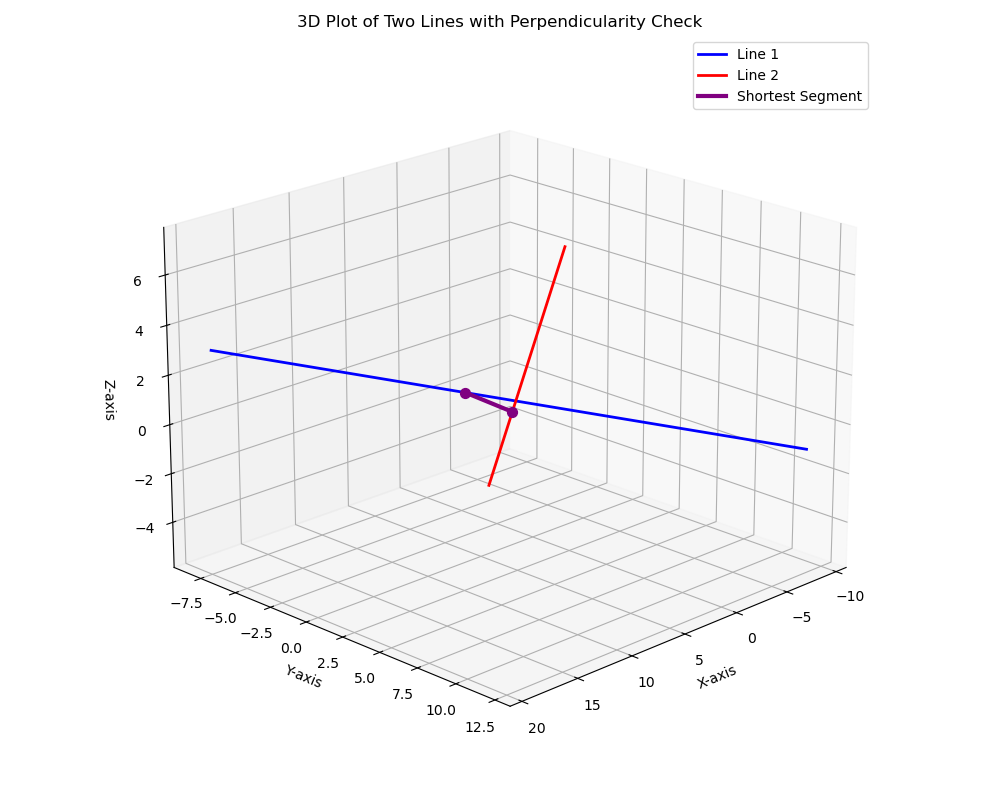
\includegraphics[width=0.9\columnwidth]{figs/fig.png}
        \caption{}
        \label{fig:placeholder}
    \end{figure}
\end{frame}
\end{document}